% Created 2022-05-17 Tue 19:36
% Intended LaTeX compiler: pdflatex
\documentclass[aspectratio=169, 10pt, handout]{beamer}
\usepackage[utf8]{inputenc}
\usepackage[T1]{fontenc}
\usepackage{graphicx}
\usepackage{longtable}
\usepackage{wrapfig}
\usepackage{rotating}
\usepackage[normalem]{ulem}
\usepackage{amsmath}
\usepackage{amssymb}
\usepackage{capt-of}
\usepackage{hyperref}
\usepackage{color}
\usepackage{listings}
\usepackage[english]{babel}
\usepackage[utf8]{inputenc}
\usepackage{roboto}
\usepackage[scaled=0.90]{roboto-mono}
\usepackage[T1]{fontenc}
\usepackage{codebeam}
\usepackage{tikz}
\usepackage{adjustbox}
\usetikzlibrary{arrows,automata,positioning}
\usetikzlibrary{overlay-beamer-styles}
\usepackage{pgfpages}
\usepackage{pgfplots}
\usepackage{listings}

\lstset{
  extendedchars=true,
  escapeinside={\#@}{\^^M},
  literate=
  {á}{{\'a}}1 {é}{{\'e}}1 {í}{{\'i}}1 {ó}{{\'o}}1 {ú}{{\'u}}1
  {Á}{{\'A}}1 {É}{{\'E}}1 {Í}{{\'I}}1 {Ó}{{\'O}}1 {Ú}{{\'U}}1
  {à}{{\`a}}1 {è}{{\`e}}1 {ì}{{\`i}}1 {ò}{{\`o}}1 {ù}{{\`u}}1
  {À}{{\`A}}1 {È}{{\'E}}1 {Ì}{{\`I}}1 {Ò}{{\`O}}1 {Ù}{{\`U}}1
  {ä}{{\"a}}1 {ë}{{\"e}}1 {ï}{{\"i}}1 {ö}{{\"o}}1 {ü}{{\"u}}1
  {Ä}{{\"A}}1 {Ë}{{\"E}}1 {Ï}{{\"I}}1 {Ö}{{\"O}}1 {Ü}{{\"U}}1
  {â}{{\^a}}1 {ê}{{\^e}}1 {î}{{\^i}}1 {ô}{{\^o}}1 {û}{{\^u}}1
  {Â}{{\^A}}1 {Ê}{{\^E}}1 {Î}{{\^I}}1 {Ô}{{\^O}}1 {Û}{{\^U}}1
  {œ}{{\oe}}1 {Œ}{{\OE}}1 {æ}{{\ae}}1 {Æ}{{\AE}}1 {ß}{{\ss}}1
  {ç}{{\c c}}1 {Ç}{{\c C}}1 {ø}{{\o}}1 {å}{{\r a}}1 {Å}{{\r A}}1
  {ñ}{~n}1
  {€}{{\EUR}}1 {£}{{\pounds}}1
  {¿}{{?`}}1 {¡}{{!`}}1 {‘}{`}1 {’}{'}1
  {·}{.}1
}

%% AH: I have tried to follow the emacs color theme jsc-light2
\usepackage{xcolor}
\definecolor{commentcolor}{rgb}{.804,0,0}
\definecolor{builtincolor}{rgb}{.855, .439, .839}
\definecolor{keywordcolor}{rgb}{.608,.19,1}
\definecolor{stringcolor}{rgb}{0,.545,0}
\definecolor{typecolor}{rgb}{0,0,.502}
\definecolor{atomcolor}{rgb}{1,.204,.70}
\definecolor{variablecolor}{rgb}{.545,.352,.17}
\definecolor{macrocolor}{rgb}{.628,.125,.94}

\lstdefinelanguage{elixir}{
    morekeywords={
      after,
      alias,
      and,
      case,
      catch,
      cond,
      def,
      defimpl,
      defmacro,
      defmacrop,
      defmodule,
      defoverridable,
      defp,
      defprotocol,
      defstruct,
      do,
      else,
      end,
      false,
      fn,
      for,
      if,
      import,
      in,
      nil,
      not,
      or,
      quote,
      raise,
      receive,
      require,
      rescue,
      true,
      try,
      unless,
      use,
      when,
      with,
      unquote,
      command,
      state,
      invariants,
      pre,
      args,
      post,
      next,
      call
    },
    emph={iex},
    alsoletter={:},
    sensitive=true,
    morecomment=[l]{\#},
    morecomment=[n]{/*}{*/},
    morecomment=[n]{@doc\ "}{"},
    morecomment=[n]{@doc\ """}{"""},
    string=[b]",
    morestring=[b]',
    showstringspaces=false
}

\lstdefinestyle{color}{
  identifierstyle=\idstyle,
  commentstyle=\itshape\color{commentcolor},
  keywordstyle=\bfseries\color{keywordcolor},
  stringstyle=\color{stringcolor},
  emphstyle=\bfseries
}

\lstdefinestyle{nocolor}{
  identifierstyle=\itshape,
  commentstyle=\itshape,
  keywordstyle=\bfseries,
  stringstyle=,
  emphstyle=\itshape
}

%% Idea for changing identifier colors taking into account :, @ and _
%% Inspiration:
%% - https://tex.stackexchange.com/questions/4198/emphasize-word-beginning-with-uppercase-letters-in-code-with-lstlisting-package)
%% - https://tex.stackexchange.com/questions/497182/highlight-all-identifiers-starting-with-an-underscore/497212#497212
%% - And package xstring
\usepackage{xstring}
\makeatletter
\newcommand*\idstyle{\expandafter\id@style\the\lst@token\relax}
\def\id@style#1#2\relax{%
  \edef\@lowline{\expandafter\noexpand\csname lst@um_\endcsname}%
  \ifcat#1%
    \relax%
  \else%
    \IfBeginWith{#1}{\@lowline}{% starts _
      \itshape\color{commentcolor}%
    }{%
      \IfBeginWith{#1}{:}{\color{atomcolor}}{}% starts :
      \IfEndWith{#2}{:}{\color{atomcolor}}{}% ends :
      \ifnum`#1=64% starts @
        \bfseries\color{builtincolor}%
      \else%
        \ifnum`#1=\uccode`#1% starts uppercase
          \itshape\color{typecolor}%
        \else%
          % default style
        \fi%
      \fi%
    }%
  \fi%
}
\makeatother

\input{listings_bash}
\lstdefinestyle{display}{style=color,basicstyle=\footnotesize\ttfamily}
\lstdefinestyle{shell}{basicstyle=\footnotesize\ttfamily}
\usetheme{default}
\author{Luis Eduardo Bueso de Barrio}
\date{\today}
\title{Improve your tests with Makina}
\hypersetup{
 pdfauthor={Luis Eduardo Bueso de Barrio},
 pdftitle={Improve your tests with Makina},
 pdfkeywords={},
 pdfsubject={},
 pdfcreator={Emacs 28.1 (Org mode 9.5.2)}, 
 pdflang={English}}
\begin{document}

\texturetheme

\setbeamertemplate{title page}{
    \begin{columns}
      \begin{column}{0.55\textwidth}
        \center
        \includegraphics[width=\textwidth]{./template/logo-white}
      \end{column}
      \begin{column}{0.40\textwidth}
        \flushright
            {\Huge STOCKHOLM}

            \vspace{0.2cm}

            {\large HYBRID CONFERENCE}

            \vspace{1cm}

            {\Large \texttt{Improve your tests with Makina}}

            \vspace{1cm}

            Luis Eduardo Bueso de Barrio

            \vspace{0.5cm}

            \texttt{May 20 | 2022}
      \end{column}
    \end{columns}
}

\maketitle

\whitetheme

\section{Motivation}
\label{sec:org90b48df}
\begin{frame}[label={sec:org1d26db6}]{}
\begin{columns}
\begin{column}{0.38\columnwidth}
Before:
\begin{center}
\begin{tabular}{rrrr}
files & blank & comment & code\\
\hline
4 & 760 & 383 & 4513\\
\end{tabular}
\end{center}
\end{column}
\begin{column}{0.38\columnwidth}
After:
\begin{center}
\begin{tabular}{rrrr}
files & blank & comment & code\\
\hline
18 & 500 & 408 & 1692\\
\end{tabular}
\end{center}
\end{column}
\end{columns}
\end{frame}

\begin{frame}[label={sec:orgfac5aa2}]{PBT models}
\begin{columns}
\begin{column}{0.48\columnwidth}
Proprety-Based Testing (PBT) is a great testing methodology.

\vspace{10pt}

Successful tools widely used:
\begin{itemize}
\item Erlang QuickCheck (EQC)
\item PropEr
\end{itemize}

\vspace{10pt}

These tools are great for testing pure functions.

\vspace{10pt}

They have mechanisms to test stateful programs.

\vspace{10pt}

PBT state-machines or models.
\end{column}

\begin{column}{0.48\columnwidth}
A PBT model is like an oracle.

\vspace{10pt}
\end{column}
\end{columns}
\end{frame}

\begin{frame}[label={sec:orgdf5c6fd}]{Problems with PBT models}
Despite their proven effectiveness:
\begin{itemize}
\item Very slow adoption
\end{itemize}

\vspace{10pt}

Why?

\vspace{10pt}

\begin{enumerate}
\item Models are hard to reuse.
\item Bugs in models are hard to detect.
\item Errors are hard to understand.
\end{enumerate}

\vspace{10pt}

All these problems made models hard to write and maintain.
\end{frame}

\section{Introduction to Makina and running example}
\label{sec:orgf41d92e}
\begin{frame}[label={sec:orga66aa88}]{Our solution: Makina}
\begin{columns}
\begin{column}{0.48\columnwidth}
Makina is a DSL for writing PBT models.

\vspace{10pt}
\end{column}

\begin{column}{0.48\columnwidth}
\begin{enumerate}
\item Models are hard to reuse.
\begin{itemize}
\item Model refinement and composition. \vspace{10pt}
\end{itemize}
\item Bugs in models are hard to detect.
\begin{itemize}
\item Automatic type and specs generation. \vspace{10pt}
\end{itemize}
\item Errors are hard to understand.
\begin{itemize}
\item Automatic generation of runtime-checks. \vspace{10pt}
\end{itemize}
\end{enumerate}
\end{column}
\end{columns}
\end{frame}

\begin{frame}[label={sec:org938edd3}]{Introduction to Makina}
\end{frame}
\begin{frame}[label={sec:orgd420cbf},fragile]{Ethereum Blockchain}
 \begin{columns}
\begin{column}{0.48\columnwidth}
\onslide<+->
\onslide<+->
A blockchain is a distributed ledger that enables peer-to-peer transactions.
\onslide<+->
\begin{figure}
\begin{adjustbox}{max width=\textwidth}
  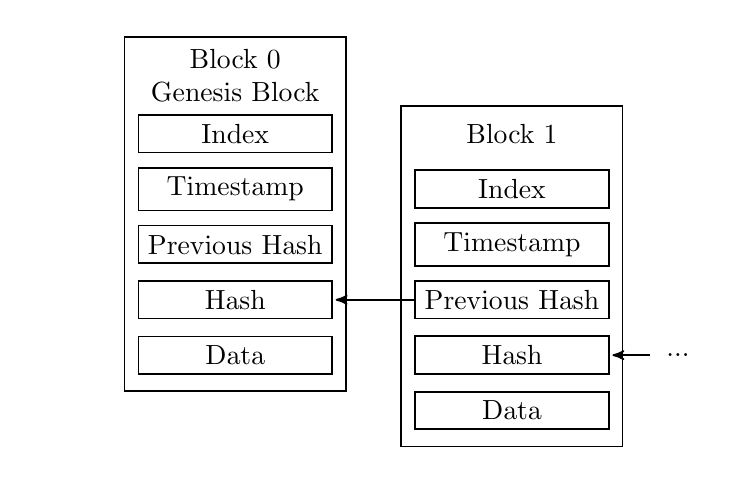
\begin{tikzpicture}[->,>=stealth',shorten >=1pt,auto,node
    distance=20,semithick, minimum width=70]

    \node (block0name) {\begin{tabular}{c} Block 0 \\ Genesis Block \end{tabular}};
    \node[rectangle, draw, below of=block0name] (block0index) {Index};
    \node[rectangle, draw, below of=block0index] (block0timestamp) {Timestamp};
    \node[rectangle, draw, below of=block0timestamp] (block0previoushash)
    {Previous Hash};
    \node[rectangle, draw, below of=block0previoushash] (block0hash)
    {Hash};
    \node[rectangle, draw, below of=block0hash] (block0data)
    {Data};

    \node [right of=block0name, yshift=-20, xshift=80] (block1name) {Block 1};
    \node[rectangle, draw, below of=block1name] (block1index) {Index};
    \node[rectangle, draw, below of=block1index] (block1timestamp) {Timestamp};
    \node[rectangle, draw, below of=block1timestamp] (block1previoushash)
    {Previous Hash};
    \node[rectangle, draw, below of=block1previoushash] (block1hash)
    {Hash};
    \node[rectangle, draw, below of=block1hash] (block1data)
    {Data};

    % \node [right of=block1name, yshift=-20, xshift=80] (block2name) {Block 2};
    % \node[rectangle, draw, below of=block2name] (block2index) {Index};
    % \node[rectangle, draw, below of=block2index] (block2timestamp) {Timestamp};
    % \node[rectangle, draw, below of=block2timestamp] (block2previoushash)
    % {Previous Hash};
    % \node[rectangle, draw, below of=block2previoushash] (block2hash)
    % {Hash};
    % \node[rectangle, draw, below of=block2hash] (block2data)
    % {Data};

    \node[right of=block1hash, xshift=40, minimum width=20] (block2previoushash)
    {...};

    \draw (block1previoushash) edge (block0hash);
    \draw (block2previoushash) edge (block1hash);

    \node[left  of=block0name, xshift=-20, yshift= 15] (block0a) {};
    \node[right of=block0data, xshift= 20, yshift=-13] (block0b) {};
    \draw[draw] (block0a) rectangle (block0b);

    \node[left  of=block1name, xshift=-20, yshift= 10] (block1a) {};
    \node[right of=block1data, xshift= 20, yshift=-13] (block1b) {};
    \draw[draw] (block1a) rectangle (block1b);

    % \node[left  of=block2name, xshift=-20, yshift= 10] (block2a) {};
    % \node[right of=block2data, xshift= 20, yshift=-10] (block2b) {};
    % \draw[draw] (block2a) rectangle (block2b);

  \end{tikzpicture}
\end{adjustbox}
\end{figure}
\end{column}

\begin{column}{0.48\columnwidth}
\onslide<+->
Why Ethereum?
\onslide<+->
\begin{itemize}
\item Big community.
\onslide<+->
\item Multiple implementations.
\onslide<+->
\end{itemize}
\vspace{10pt}

To interact we will use \texttt{etherex}:
\onslide<+->
\url{https://gitlab.com/babel-upm/blockchain/etherex}

\onslide<+->
\vspace{10pt}

The properties to test:
\onslide<+->
\begin{enumerate}
\item Mining blocks.
\onslide<+->
\item Account access.
\onslide<+->
\item Transactions between accounts.
\end{enumerate}
\end{column}
\end{columns}
\end{frame}

\section{Blocks model}
\label{sec:orge32723c}
\begin{frame}[label={sec:orga9b7c60},fragile]{Mining blocks}
 \begin{columns}
\begin{column}{0.48\columnwidth}
\onslide<+->
\onslide<+->
The API:
\onslide<+->
\begin{center}
\begin{tabular}{ll}
Command & Returns\\
\hline
\texttt{mine/0} & \texttt{:ok}\\
\texttt{block\_number/0} & \texttt{integer()}\\
\end{tabular}
\end{center}
\onslide<+->
\vspace{10pt}
\begin{enumerate}
\item create module.
\onslide<+->
\item import \texttt{Makina}.
\onslide<+->
\item define state.
\onslide<+->
\item define invariants.
\onslide<+->
\item define commands.
\end{enumerate}
\end{column}

\begin{column}{0.48\columnwidth}
\onslide<4->
\lstset{language=elixir,label= ,caption= ,captionpos=b,numbers=none,style=display}
\begin{lstlisting}
defmodule Blocks do #@ \onslide<5->
  use Makina
  #@ \onslide<6->
  state height: 0
  #@ \onslide<7->
  invariants non_neg_height: height > 0
  #@ \onslide<8->
  command block_number() do #@ \onslide<9->
    pre true #@ \onslide<10->
    args [] #@ \onslide<11->
    call Etherex.block_number #@ \onslide<12->
    next [] #@ \onslide<13->
    post height == result #@ \onslide<14->
  end
\end{lstlisting}
\end{column}
\end{columns}
\end{frame}

\begin{frame}[label={sec:org8dfff0c},fragile]{Mining blocks}
 \begin{columns}
\begin{column}{0.48\columnwidth}
The API:

\begin{center}
\begin{tabular}{ll}
Command & Returns\\
\hline
\texttt{mine/0} & \texttt{:ok}\\
\texttt{block\_number/0} & \texttt{integer()}\\
\end{tabular}
\end{center}

\vspace{10pt}
\begin{enumerate}
\item create module.
\item import \texttt{Makina}.
\item define state.
\item define invariants.
\item define commands.
\end{enumerate}
\end{column}

\begin{column}{0.48\columnwidth}
\lstset{language=elixir,label= ,caption= ,captionpos=b,numbers=none,style=display}
\begin{lstlisting}
defmodule Blocks do
  use Makina, implemented_by: Etherex

  state height: 0

  invariants non_neg_height: height > 0

  command block_number() do
    post height == result
  end
  #@ \onslide<2->
  command mine() do
    next height: height + 1
  end
end
\end{lstlisting}
\end{column}
\end{columns}
\end{frame}

\begin{frame}[label={sec:org501af93},fragile]{Running the test}
 \begin{columns}
\begin{column}{0.48\columnwidth}
\onslide<+->
\lstset{language=bash,label= ,caption= ,captionpos=b,numbers=none,style=shell}
\begin{lstlisting}
$ mix test
#@ \onslide<+->
Failed! After 1 tests.

Postcondition crashed:
** invariant "non_neg_height" check failed

Shrinking x.(1 times)
[
    Blocks.block_number/0
]

Last state: %{height: 0}
\end{lstlisting}
\end{column}

\begin{column}{0.48\columnwidth}
\onslide<1->
\lstset{language=elixir,label= ,caption= ,captionpos=b,numbers=none,style=display}
\begin{lstlisting}
defmodule Blocks do
  use Makina, implemented_by: Etherex

  state height: 0

  invariants non_neg_height: height > 0

  command block_number() do
    post height == result
  end

  command mine() do
    next height: height + 1
  end
end
\end{lstlisting}
\end{column}
\end{columns}
\end{frame}

\begin{frame}[label={sec:org7ca0fae},fragile]{Fixing the model}
 \begin{columns}
\begin{column}{0.48\columnwidth}
\onslide<+->
\lstset{language=bash,label= ,caption= ,captionpos=b,numbers=none,style=shell}
\begin{lstlisting}
$ mix test

Failed! After 1 tests.

Postcondition crashed:
** invariant "non_neg_height" check failed

Shrinking x.(1 times)
[
    Blocks.block_number/0
]

Last state: %{height: 0}
\end{lstlisting}
\end{column}

\begin{column}{0.48\columnwidth}
\lstset{language=elixir,label= ,caption= ,captionpos=b,numbers=none,style=display}
\begin{lstlisting}
defmodule Blocks do
  use Makina, implemented_by: Etherex

  state height: 0

  invariants non_neg_height: height >#@\only<2->{=} 0

  command block_number() do
    post height == result
  end

  command mine() do
    next height: height + 1
  end
end
\end{lstlisting}
\end{column}
\end{columns}
\end{frame}

\begin{frame}[label={sec:orgee404b5},fragile]{Running the test}
 \begin{columns}
\begin{column}{0.48\columnwidth}
\lstset{language=bash,label= ,caption= ,captionpos=b,numbers=none,style=shell}
\begin{lstlisting}
$ mix test #@\onslide<+->
#@\onslide<+->
..................................................
..................................................

OK, passed 100 tests

51.5 Blocks.mine/0
48.5 Blocks.block_number/0
\end{lstlisting}
\end{column}

\begin{column}{0.48\columnwidth}
\onslide<1->
\lstset{language=elixir,label= ,caption= ,captionpos=b,numbers=none,style=display}
\begin{lstlisting}
defmodule Blocks do
  use Makina, implemented_by: Etherex

  state height: 0

  invariants non_neg_height: height >= 0

  command block_number() do
    post height == result
  end

  command mine() do
    next height: height + 1
  end
end
\end{lstlisting}
\end{column}
\end{columns}
\end{frame}

\begin{frame}[label={sec:orgff89665},fragile]{Adding type information}
 \begin{columns}
\begin{column}{0.48\columnwidth}
\onslide<3->
\lstset{language=bash,label= ,caption= ,captionpos=b,numbers=none,style=shell}
\begin{lstlisting}
$ mix gradient

$
\end{lstlisting}

\vspace{10pt}
\onslide<4->
Something changes in \texttt{Etherex}\ldots{}

\vspace{10pt}

\onslide<5->
\lstset{language=bash,label= ,caption= ,captionpos=b,numbers=none,style=shell}
\begin{lstlisting}
$ mix gradient

The function call Etherex.block_number()
on line 8 is expected to have type integer()
but it has type
{:ok, quantity()} | {:error, error()}

$
\end{lstlisting}
\end{column}

\begin{column}{0.48\columnwidth}
\onslide<1->
\lstset{language=elixir,label= ,caption= ,captionpos=b,numbers=none,style=display, numbers=left}
\begin{lstlisting}
defmodule Blocks do
  use Makina, implemented_by: Etherex

  state height: 0 #@\only<2->{:: integer()}

  invariants non_neg_height: height >= 0

  command block_number()#@\only<2->{ :: integer()} do
    post height == result
  end

  command mine()#@\only<2->{ :: :ok} do
    next height: height + 1
  end
end
\end{lstlisting}
\end{column}
\end{columns}
\end{frame}

\begin{frame}[label={sec:org5758c4e},fragile]{Adding documentation}
 \begin{columns}
\begin{column}{0.48\columnwidth}
\onslide<3->
\lstset{language=bash,label= ,caption= ,captionpos=b,numbers=none,style=shell}
\begin{lstlisting}
iex> h Blocks
#@\onslide<4->
Contains a Makina model called Blocks.

Checks blocks are mined correctly.

## Commands

- mine stored at Blocks.Command.Mine
- block_number stored at Blocks.Command.BlockNumber

## State attributes

- height

## Invariants

- non_neg_height
\end{lstlisting}
\end{column}

\begin{column}{0.48\columnwidth}
\onslide<1->
\lstset{language=elixir,label= ,caption= ,captionpos=b,numbers=none,style=display}
\begin{lstlisting}
defmodule Blocks do
  use Makina, implemented_by: Etherex
  #@ \onslide<2->
  @moduledoc """
  Checks blocks are mined correctly.
  """ #@ \onslide<1->
  state height: 0 :: integer()

  invariants non_neg_height: height >= 0

  command block_number() :: integer() do #@ \onslide<2->
    @moduledoc "Gets the block number." #@ \onslide<1->
    post {:ok, height} == result
  end

  command mine() :: :ok do #@ \onslide<2->
    @moduledoc "Mines a new block." #@ \onslide<1->
    next height: height + 1
  end
end
\end{lstlisting}
\end{column}
\end{columns}
\end{frame}

\begin{frame}[label={sec:orga2a0473},fragile]{Adding documentation}
 \begin{columns}
\begin{column}{0.48\columnwidth}
\onslide<1->
\lstset{language=bash,label= ,caption= ,captionpos=b,numbers=none,style=shell}
\begin{lstlisting}
iex> h Blocks.Command.Mine
#@\onslide<2->
This module contains the functions necessary to
generate and execute the command mine.

Mines a new block.

## Definitions

- next
- call
- weight
- post
- args
- pre
\end{lstlisting}
\end{column}

\begin{column}{0.48\columnwidth}
\onslide<1->
\lstset{language=elixir,label= ,caption= ,captionpos=b,numbers=none,style=display}
\begin{lstlisting}
defmodule Blocks do
  use Makina, implemented_by: Etherex

  @moduledoc """
  Checks blocks are mined correctly.
  """
  state height: 0 :: integer()

  invariants non_neg_height: height >= 0

  command block_number() :: integer() do
    @moduledoc "Gets the block number."
    post {:ok, height} == result
  end

  command mine() :: :ok do
    @moduledoc "Mines a new block."
    next height: height + 1
  end
end
\end{lstlisting}
\end{column}
\end{columns}
\end{frame}

\begin{frame}[label={sec:orgfb6acf8},fragile]{Adding documentation}
 \begin{columns}
\begin{column}{0.48\columnwidth}
\onslide<1->
\lstset{language=bash,label= ,caption= ,captionpos=b,numbers=none,style=shell}
\begin{lstlisting}
iex> h Blocks.Command.Mine.post
#@\onslide<2->
This definition contains a predicate that should
be true after the execution of mine

## Available variables

### State

  - state
  - height

### Arguments

  - arguments

### Result

  - result
\end{lstlisting}
\end{column}

\begin{column}{0.48\columnwidth}
\onslide<1->
\lstset{language=elixir,label= ,caption= ,captionpos=b,numbers=none,style=display}
\begin{lstlisting}
defmodule Blocks do
  use Makina, implemented_by: Etherex

  @moduledoc """
  Checks blocks are mined correctly.
  """
  state height: 0 :: integer()

  invariants non_neg_height: height >= 0

  command block_number() :: integer() do
    @moduledoc "Gets the block number."
    post {:ok, height} == result
  end

  command mine() :: :ok do
    @moduledoc "Mines a new block."
    next height: height + 1
  end
end
\end{lstlisting}
\end{column}
\end{columns}
\end{frame}

\section{Accounts model}
\label{sec:org14eaa08}
\begin{frame}[label={sec:orgbf2ad66},fragile]{Account access}
 \begin{columns}
\begin{column}{0.28\columnwidth}
\onslide<+->
The API:

\begin{center}
\begin{tabular}{ll}
Command & Returns\\
\hline
\texttt{balance/1} & \texttt{integer()}\\
\end{tabular}
\end{center}
\onslide<+->
\vspace{0.5cm}
\begin{enumerate}
\item create module.
\onslide<+->
\item import \texttt{Makina}.
\onslide<+->
\item define state.
\onslide<+->
\item define commands.
\end{enumerate}
\end{column}

\begin{column}{0.58\columnwidth}
\onslide<2->
\lstset{language=elixir,label= ,caption= ,captionpos=b,numbers=none,style=display}
\begin{lstlisting}
defmodule Accounts do #@\onslide<3->
  use Makina, implemented_by: Etherex
  #@\onslide<4->
  state accounts: Etherex.accounts() :: [address()],
	balances: Etherex.balances() :: %{address() => integer()}
  #@\onslide<5->
  command balance(account :: address()) :: integer() do
    pre accounts != []
    post balances[account] == result
  end #@\onslide<2->
end
\end{lstlisting}
\end{column}
\end{columns}
\end{frame}

\begin{frame}[label={sec:org5809e5c},fragile]{Running the test}
 \begin{columns}
\begin{column}{0.28\columnwidth}
\onslide<+->
\lstset{language=bash,label= ,caption= ,captionpos=b,numbers=none,style=shell}
\begin{lstlisting}
$ mix test
#@\onslide<+->
** (Makina.Error) argument
    `account` missing in command
    get_balance
\end{lstlisting}
\vspace{40pt}
\end{column}

\begin{column}{0.58\columnwidth}
\onslide<1->
\lstset{language=elixir,label= ,caption= ,captionpos=b,numbers=none,style=display}
\begin{lstlisting}
defmodule Accounts do
  use Makina, implemented_by: Etherex

  state accounts: Etherex.accounts() :: [address()],
	balances: Etherex.balances() :: %{address() => integer()}

  command balance(account :: address()) :: integer() do
    pre accounts != []
    post balances[account] == result
  end
end
\end{lstlisting}
\end{column}
\end{columns}
\end{frame}

\begin{frame}[label={sec:org1de2016},fragile]{Fixing the model}
 \begin{columns}
\begin{column}{0.28\columnwidth}
\onslide<+->
\lstset{language=bash,label= ,caption= ,captionpos=b,numbers=none,style=shell}
\begin{lstlisting}
$ mix test

** (Makina.Error) argument
    `account` missing in command
    get_balance
\end{lstlisting}
\vspace{40pt}
\end{column}

\begin{column}{0.58\columnwidth}
\onslide<1->
\lstset{language=elixir,label= ,caption= ,captionpos=b,numbers=none,style=display}
\begin{lstlisting}
defmodule Accounts do
  use Makina, implemented_by: Etherex

  state accounts: Etherex.accounts() :: [address()],
	balances: Etherex.balances() :: %{address() => integer()}

  command balance(account :: address()) :: integer() do
    args account: oneof(accounts)
    pre accounts != []
    post balances[account] == result
  end
end
\end{lstlisting}
\end{column}
\end{columns}
\end{frame}

\begin{frame}[label={sec:org2b4aa8b},fragile]{Running the test}
 \begin{columns}
\begin{column}{0.28\columnwidth}
\lstset{language=bash,label= ,caption= ,captionpos=b,numbers=none,style=shell}
\begin{lstlisting}
$ mix test #@\onslide<+->
#@\onslide<+->
.........................
.........................
.........................
.........................
OK, passed 100 tests

'100.0 Accounts.get_balance/1
\end{lstlisting}
\end{column}

\begin{column}{0.58\columnwidth}
\onslide<1->
\lstset{language=elixir,label= ,caption= ,captionpos=b,numbers=none,style=display}
\begin{lstlisting}
defmodule Accounts do
  use Makina, implemented_by: Etherex

  state accounts: Etherex.accounts() :: [address()],
	balances: Etherex.balances() :: %{address() => integer()}

  command balance(account :: address()) :: integer() do
    args account: oneof(accounts)
    pre accounts != []
    post balances[account] == result
  end
end
\end{lstlisting}
\end{column}
\end{columns}
\end{frame}

\section{Transactions model}
\label{sec:org66f5463}
\begin{frame}[label={sec:orgd1afc9d},fragile]{Generating transactions}
 \begin{columns}
\begin{column}{0.48\columnwidth}
\onslide<+->
\onslide<+->
The API to generate and check transactions:
\onslide<+->
\begin{center}
\begin{tabular}{ll}
Command & Returns\\
\hline
\texttt{mine/0} & \texttt{:ok}\\
\texttt{block\_number/0} & \texttt{integer()}\\
\texttt{get\_balance/1} & \texttt{integer()}\\
\texttt{transfer/3} & \texttt{hash()}\\
\end{tabular}
\end{center}
\onslide<+->
We can compose \texttt{Blocks} and \texttt{Accounts}!
\onslide<+->
\lstset{language=elixir,label= ,caption= ,captionpos=b,numbers=none,style=display}
\begin{lstlisting}
defmodule Transactions do
  use Makina,
    extends: [Blocks, Accounts],
    implemented_by: Etherex
end
\end{lstlisting}
\onslide<+->
Generates a model \texttt{Transactions.Composed}.
\end{column}

\begin{column}{0.48\columnwidth}
\onslide<+->
\lstset{language=bash,label= ,caption= ,captionpos=b,numbers=none,style=shell}
\begin{lstlisting}
iex(1)> h Transactions.Composed
#@\onslide<+->
# Transactions.Composed

## Commands

 - mine stored
 - get_balance
 - block_number

## State attributes

 - height
 - balances
 - accounts

## Invariants

 - non_neg_height

\end{lstlisting}
\end{column}
\end{columns}
\end{frame}

\begin{frame}[label={sec:org7f823e6},fragile]{Generating transactions}
 \begin{columns}
\begin{column}{0.44\columnwidth}
\onslide<+->
\begin{center}
\begin{tabular}{ll}
Command & Returns\\
\hline
\texttt{transfer/3} & \texttt{hash()}\\
\end{tabular}
\end{center}
\end{column}
\begin{column}{0.52\columnwidth}
\onslide<+->
\lstset{language=elixir,label= ,caption= ,captionpos=b,numbers=none,style=display}
\begin{lstlisting}
defmodule Transactions do
  use Makina,
    implemented_by: Etherex,
    extends: [Accounts, Blocks]

  command transfer(from, to, value) :: hash() do
    pre accounts != []
    args from: oneof(accounts),
	 to: oneof(accounts),
	 value: pos_integer()
    next balances: update(balances, from, to, value)
  end
end
\end{lstlisting}
\end{column}
\end{columns}
\end{frame}

\begin{frame}[label={sec:orgf92c75f},fragile]{Running the test}
 \begin{columns}
\begin{column}{0.44\columnwidth}
\lstset{language=bash,label= ,caption= ,captionpos=b,numbers=none,style=shell}
\begin{lstlisting}
$ mix test #@\onslide<+->

transfer("0xffcf8fdee72ac11",
	 "0x90f8bf6a479f320",
	 1)
block_number()

Postcondition failed.

block_number() -> {:ok, 1}

Last state: %{height: 0, ...}
\end{lstlisting}
\end{column}

\begin{column}{0.52\columnwidth}
\onslide<+->
\lstset{language=elixir,label= ,caption= ,captionpos=b,numbers=none,style=display}
\begin{lstlisting}
defmodule Transactions do
  use Makina,
    implemented_by: Etherex,
    extends: [Accounts, Blocks]

  command transfer(from, to, value) :: hash() do
    pre accounts != []
    args from: oneof(accounts),
	 to: oneof(accounts),
	 value: pos_integer()
    next balances: update(balances, from, to, value)
  end
end
\end{lstlisting}
\end{column}
\end{columns}
\end{frame}

\begin{frame}[label={sec:orga87c4c1},fragile]{Fixing the model}
 \begin{columns}
\begin{column}{0.44\columnwidth}
\lstset{language=bash,label= ,caption= ,captionpos=b,numbers=none,style=shell}
\begin{lstlisting}
$ mix test #@\onslide<+->

Postcondition failed.

transfer("0xffcf8fdee72ac11",
	 "0x90f8bf6a479f320",
	 1)
block_number() -> {:ok, 1}

Last state: %{height: 0, ...}
\end{lstlisting}
\end{column}

\begin{column}{0.52\columnwidth}
\onslide<+->
\lstset{language=elixir,label= ,caption= ,captionpos=b,numbers=none,style=display}
\begin{lstlisting}
defmodule Transactions do
  use Makina,
    implemented_by: Etherex,
    extends: [Accounts, Blocks]

  command transfer(from, to, value) :: hash() do
    pre accounts != []
    args from: oneof(accounts),
	 to: oneof(accounts),
	 value: pos_integer()
    next height: height + 1,
	 balances: update(balances, from, to, value)
  end
end
\end{lstlisting}
\end{column}
\end{columns}
\end{frame}

\begin{frame}[label={sec:orgd72411c},fragile]{Running the test}
 \begin{columns}
\begin{column}{0.44\columnwidth}
\lstset{language=bash,label= ,caption= ,captionpos=b,numbers=none,style=shell}
\begin{lstlisting}
$ mix test #@\onslide<+->

transfer("0x90f8bf6a479f320",
	 "0x90f8bf6a479f320",
	 1),
get_balance("0x90f8bf6a479f320")

Postcondition failed.

get_balance("0x90f8bf6a479f320")
-> {:ok, 979000}

Last state: %{
    balances: %{
	"0x90f8bf6a479f320" => 1000000
	.. }
    .. }
\end{lstlisting}
\end{column}

\begin{column}{0.52\columnwidth}
\onslide<+->
\lstset{language=elixir,label= ,caption= ,captionpos=b,numbers=none,style=display}
\begin{lstlisting}
defmodule Transactions do
  use Makina,
    implemented_by: Etherex,
    extends: [Accounts, Blocks]

  command transfer(from, to, value) :: hash() do
    pre accounts != []
    args from: oneof(accounts),
	 to: oneof(accounts),
	 value: pos_integer()
    next height: height + 1,
	 balances: update(balances, from, to, value)
  end
end
\end{lstlisting}
\end{column}
\end{columns}
\end{frame}

\begin{frame}[label={sec:org6cea16a},fragile]{Fixing the model}
 \begin{columns}
\begin{column}{0.44\columnwidth}
\end{column}
\begin{column}{0.52\columnwidth}
\onslide<+->
\lstset{language=elixir,label= ,caption= ,captionpos=b,numbers=none,style=display}
\begin{lstlisting}
defmodule Transactions do
  use Makina,
    implemented_by: Etherex,
    extends: [Accounts, Blocks]

  command transfer(from, to, value) :: hash() do
    pre accounts != []
    args from: oneof(accounts),
	 to: oneof(accounts),
	 value: pos_integer()
    next height: height + 1,
	 balances: update(balances, from, to, value)
  end
end
\end{lstlisting}
\end{column}
\end{columns}
\end{frame}

\begin{frame}[label={sec:org897a3f9},fragile]{Fixing the model}
 \begin{columns}
\begin{column}{0.44\columnwidth}
\end{column}

\begin{column}{0.52\columnwidth}
\onslide<+->
\vspace{-10pt}
\lstset{language=elixir,label= ,caption= ,captionpos=b,numbers=none,style=display}
\begin{lstlisting}
defmodule Transactions do
  use Makina,
    implemented_by: Etherex,
    extends: [Accounts, Blocks]

  state transactions: [] :: [symbolic(hash())]

  command transfer(from, to, value) :: hash() do
    pre accounts != []
    args from: oneof(accounts),
	 to: oneof(accounts),
	 value: pos_integer()
    next height: height + 1,
	 transactions: [result | transactions],
	 balances: update(balances, from, to, value)
		   |> symbolic(),
  end

  command get_balance() do
    pre transactions == []
  end
end
\end{lstlisting}
\end{column}
\end{columns}
\end{frame}

\begin{frame}[label={sec:org46c24a6},fragile]{Fixing the model}
 \begin{columns}
\begin{column}{0.44\columnwidth}
\end{column}

\begin{column}{0.52\columnwidth}
\lstset{language=elixir,label= ,caption= ,captionpos=b,numbers=none,style=display}
\begin{lstlisting}
defmodule Transactions.GasCost do
  use Makina, extends: Transactions

  command gas_cost(hash :: hash())
      :: {address(), quantity()} do
    pre transactions != []
    args hash: oneof(transactions)
    next do
      from = symbolic(elem(result, 0))
      gas = symbolic(elem(result, 1))
      [transactions: List.delete(transactions, hash),
       balances: update(balances, from, gas)
		 |> symbolic()
      ]
    end
  end
end
\end{lstlisting}
\end{column}
\end{columns}
\end{frame}

\begin{frame}[label={sec:org369b4b0},fragile]{Running the test}
 \begin{columns}
\begin{column}{0.44\columnwidth}
\lstset{language=bash,label= ,caption= ,captionpos=b,numbers=none,style=shell}
\begin{lstlisting}
$ mix test

..................................................
..................................................
OK, passed 100 tests

'25.5 Transactions.mine/0
'24.9 Transactions.block_number/0
'23.6 Transactions.transfer/3
'14.3 Transactions.gas_cost/1
'11.8 Transactions.get_balance/1
\end{lstlisting}
\end{column}

\begin{column}{0.52\columnwidth}
\lstset{language=elixir,label= ,caption= ,captionpos=b,numbers=none,style=display}
\begin{lstlisting}
defmodule Transactions.GasCost do
  use Makina, extends: Transactions

  command gas_cost(hash :: hash())
      :: {address(), quantity()} do
    pre transactions != []
    args hash: oneof(transactions)
    next do
      from = symbolic(elem(result, 0))
      gas = symbolic(elem(result, 1))
      [transactions: List.delete(transactions, hash),
       balances: update(balances, from, gas)
		 |> symbolic()
      ]
    end
  end
end
\end{lstlisting}
\end{column}
\end{columns}
\end{frame}
\section{Conclusions}
\label{sec:orgdd9b0e6}
\begin{frame}[label={sec:orgbcd753f}]{Results and conclussions}
\begin{columns}
\begin{column}{0.38\columnwidth}
Before Makina:
\begin{center}
\begin{tabular}{rrrr}
files & blank & comment & code\\
\hline
4 & 760 & 383 & 4513\\
\end{tabular}
\end{center}

\vspace{10pt}

After Makina:
\begin{center}
\begin{tabular}{rrrr}
files & blank & comment & code\\
\hline
18 & 500 & 408 & 1692\\
\end{tabular}
\end{center}
\end{column}

\begin{column}{0.58\columnwidth}
Libraries:
\begin{itemize}
\item \url{https://gitlab.com/babel-upm/makina/makina}
\item \url{https://gitlab.com/babel-upm/blockchain/etherex}
\end{itemize}

Slides and code:  
\begin{itemize}
\item \url{https://gitlab.com/babel-upm/makina/code\_beam\_2022}
\end{itemize}
\end{column}
\end{columns}
\end{frame}
\end{document}